\documentclass[a4paper, 11pt]{article} % Uses article class in A4 format

%----------------------------------------------------------------------------------------
%	FORMATTING
%----------------------------------------------------------------------------------------

\addtolength{\hoffset}{-2.25cm}
\addtolength{\textwidth}{4.5cm}
\addtolength{\voffset}{-3.25cm}
\addtolength{\textheight}{5cm}
\setlength{\parskip}{1.5ex}
\setlength{\parindent}{0em}

%----------------------------------------------------------------------------------------
%	PACKAGES AND OTHER DOCUMENT CONFIGURATIONS
%----------------------------------------------------------------------------------------

\usepackage{charter} % Use the Charter font
\usepackage[utf8]{inputenc} % Use UTF-8 encoding
\usepackage{microtype} % Slightly tweak font spacing for aesthetics

\usepackage[english]{babel} % Language hyphenation and typographical rules

\usepackage{amsthm, amsmath, amssymb} % Mathematical typesetting
\usepackage{float} % Improved interface for floating objects
\usepackage[final, colorlinks = true, 
            linkcolor = black, 
            citecolor = black]{hyperref} % For hyperlinks in the PDF
\usepackage{graphicx, multicol} % Enhanced support for graphics
\usepackage{color}
\usepackage{xcolor} % Driver-independent color extensions
\usepackage{marvosym, wasysym} % More symbols
\usepackage{rotating} % Rotation tools
\usepackage{censor} % Facilities for controlling restricted text
\usepackage{listings} % Environment for non-formatted code
\usepackage{algorithm}
\usepackage{algpseudocode} % Environment for specifying algorithms in a natural way
\usepackage{booktabs} % Enhances quality of tables

\usepackage{cases}
\usepackage{bookmark}

\usepackage{tikz-qtree} % Easy tree drawing tool
\tikzset{every tree node/.style={align=center,anchor=north},
         level distance=2cm} % Configuration for q-trees

\usepackage[backend=biber,style=numeric,
            sorting=nyt]{biblatex} % Complete reimplementation of bibliographic facilities

\usepackage{csquotes} % Context sensitive quotation facilities

\usepackage[yyyymmdd]{datetime} % Uses YEAR-MONTH-DAY format for dates
\renewcommand{\dateseparator}{-} % Sets dateseparator to '-'

\usepackage{fancyhdr} % Headers and footers
\pagestyle{fancy} % All pages have headers and footers
\fancyhead{}\renewcommand{\headrulewidth}{0pt} % Blank out the default header
\fancyfoot[L]{} % Custom footer text
\fancyfoot[C]{} % Custom footer text
\fancyfoot[R]{\thepage} % Custom footer text

\newcommand{\note}[1]{\marginpar{\scriptsize \textcolor{red}{#1}}} % Enables comments in red on margin


\lstset{ %
	language=python,                % choose the language of the code
	basicstyle=\footnotesize\ttfamily,       % the size of the fonts that are used for the code
	numbers=left,                   % where to put the line-numbers
	numberstyle=\tiny\color{blue},      % the size of the fonts that are used for the line-numbers
	stepnumber=1,                   % the step between two line-numbers. If it is 1 each line will be numbered
	numbersep=5pt,                  % how far the line-numbers are from the code
	backgroundcolor=\color{white},  % choose the background color. You must add \usepackage{color}
	showspaces=false,               % show spaces adding particular underscores
	showstringspaces=false,         % underline spaces within strings
	showtabs=false,                 % show tabs within strings adding particular underscores
	frame=single,                   % adds a frame around the code
	tabsize=4,                      % sets default tabsize to 4 spaces  
	captionpos=b,                   % sets the caption-position to bottom
	breaklines=true,                % sets automatic line breaking
	breakatwhitespace=false,        % sets if automatic breaks should only happen at whitespace
	escapeinside={\%*}{*)},
	commentstyle=\color{gray},
	keywordstyle=\bfseries\color{red},
	stringstyle=\color{orange},
	keepspaces=true
}

%----------------------------------------------------------------------------------------

\begin{document}

%----------------------------------------------------------------------------------------
%	TITLE SECTION
%----------------------------------------------------------------------------------------

\fancyhead[C]{}
\hrule \medskip % Upper rule
\begin{minipage}{0.295\textwidth} % Left side of title section
    \raggedright
    DATA130011.01\\ % Your course code
    \footnotesize % Authors text size
    \hfill\\
    Neural Network and Deep Learning\\ % Your course name
\end{minipage}
\begin{minipage}{0.4\textwidth} % Center of title section
    \centering
    \large % Title text size
    \textbf{Project I}\\ % Assignment title and number
    \normalsize % Subtitle text size
    \textbf{Latte}\\ % Assignment subtitle
\end{minipage}
\begin{minipage}{0.295\textwidth} % Right side of title section
    \raggedleft
    Shao Yi\\ % Your name
    \footnotesize % Email text size
    \hfill\\
    \today\\ % Date
\end{minipage}
\medskip\hrule % Lower rule
\bigskip

%----------------------------------------------------------------------------------------
%	ARTICLE CONTENTS
%----------------------------------------------------------------------------------------

\section*{\textbf{Abstract}}

\textbf{Latte} (\textbf{L}et's \textbf{A}bsorb \textbf{T}orch \textbf{T}echnology
\textbf{E}legantly) is a self-designed deep learning framework working on CPU, the package
name shows tribute to Caffe while the inner structure is inspired by the PyTorch framework.
This project focuses on the manual implementation of the most common deep learning package
modules and solves the \textbf{MNIST} dataset classification problem.

\bigskip

%------------------------------------------------

\section{\textbf{Introduction}}

The package structure in the tree view is as follows:

\begin{figure}[H]
    \centering
    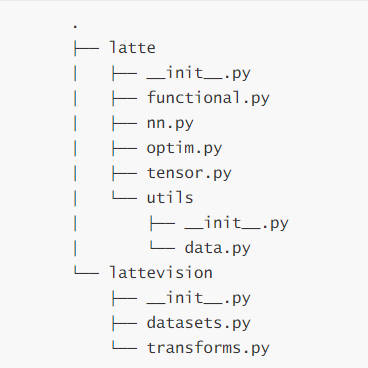
\includegraphics[width=0.4\textwidth]{./img/tree.jpg}
    \caption{Package Structure}
\end{figure}

Latte packages some basic modules, like \textbf{tensor} defines the basic data structure,
\textbf{nn} together with \textbf{functional} provides necessary classes and functions
for neural network, \textbf{optim} includes some classical optimization methods, and
\textbf{utils.data} is for dataset and data loader. All the interfaces are referred to
the official documentation of PyTorch.

Furthermore, what torchvision is to torch, lattevision is to latte. It includes some
requisite modules for computer vision tasks. To be more specific, \textbf{transforms}
contains some transformation functions for image processing, \textbf{datasets} implements
the downloading and loading of MNIST dataset for now.

All the features above are implemented using \textbf{numpy} package.

\subsection{\textbf{Dataset}}

Imitating the PyTorch \textbf{torchvision.datasets} module, we implement \textbf{MNIST},
the core code is shown below, for more details please refer to source code.

\begin{lstlisting}
class MNIST(VisionDataset):
    def __init__(
        self,
        root: str,
        train: bool = True,
        transform: Optional[Callable] = None,
        target_transform: Optional[Callable] = None,
    ) -> None:
        super().__init__(root, train, transform, target_transform)

    def _load_dataset(self) -> None:
        url = 'http://yann.lecun.com/exdb/mnist/'
        if self.train:
            data_filename = 'train-images-idx3-ubyte.gz'
            labels_filename = 'train-labels-idx1-ubyte.gz'
        else:
            data_filename = 't10k-images-idx3-ubyte.gz'
            labels_filename = 't10k-labels-idx1-ubyte.gz'

        data_filepath = get_data(url + data_filename, self.root)
        labels_filepath = get_data(url + labels_filename, self.root)

        self.data = self._load_data(data_filepath)
        self.labels = self._load_labels(labels_filepath)

    def _load_data(self, filepath: str) -> np.ndarray:
        with gzip.open(filepath, 'rb') as f:
            data = np.frombuffer(f.read(), np.uint8, offset=16)
        data = data.reshape(-1, 1, 28, 28)
        return data

    def _load_labels(self, filepath: str) -> np.ndarray:
        with gzip.open(filepath, 'rb') as f:
            labels = np.frombuffer(f.read(), np.uint8, offset=8)
        return labels
\end{lstlisting}

Therefore, all the network training is based on the official MNIST dataset instead of our
16*16 version.

\subsection{\textbf{Computational Graph}}

In the \textbf{tensor} module, building computational graph is wrapped in the backward
function of \textbf{Tensor} class in order to support the backpropagation, the corresponding
code is as follows:

\begin{lstlisting}
class Tensor:
def __init__(
		self,
		data: np.ndarray,
		grad_fn: 'Function' = None,
		requires_grad: bool = False,
		is_bias: bool = False,  # Notation for bias, not official
	) -> None:
		pass

	# More specifications can be found in the source code

	def backward(self) -> None:
	    # Build computational graph
        graph = []
        visited = set()

        def build_graph(node: 'Tensor'):
            if node.requires_grad is True and node not in visited:
                visited.add(node)

                # Post-order traversal
                if node.grad_fn is not None:
                    for prev_node in node.grad_fn.prev:
                        build_graph(prev_node)

                graph.append(node)

        build_graph(self)

        # Backpropagate gradients
        self.grad = np.array([1.0]).reshape(1, 1)  # Create implicit gradient
        for node in reversed(graph):
            if node.grad_fn is not None:
                node.grad_fn.backward(node.grad)
\end{lstlisting}

Besides, every single \textbf{basic operation} in our arithmetic library is implemented
with the \textbf{backward function}. In this way, we can basically reproduce PyTorch's
propagation mechanism.

\subsection{\textbf{Quick Start}}

This part is a quick start guide, we run a toy example to see how the framework works. By
the way, all the code implementations are included in jupyter notebooks.

The nerwork architecture is shown in the following figure:

\begin{figure}[H]
    \centering
    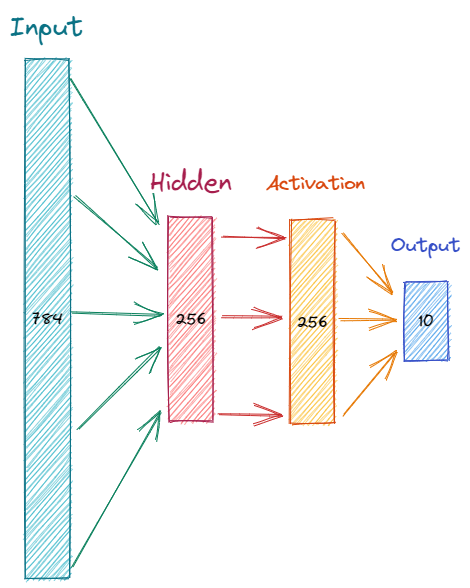
\includegraphics[width=0.5\textwidth]{./img/simple-network.png}
    \caption{Simple Network}
\end{figure}

As an example, we use only \textbf{fully connected} layers to build a simple network, the
activation function is \textbf{ReLU}. For criterion and optimizer, we use \textbf{CrossEntropyLoss}
and \textbf{Adam} respectively.

The training result should be good because we already apply some advanced techniques in
this example, so we just set training epochs to 5 and learning rate so as to 0.001 to see
if the framework works. And here is the visualization of training process:

\begin{figure}[H]
    \centering
    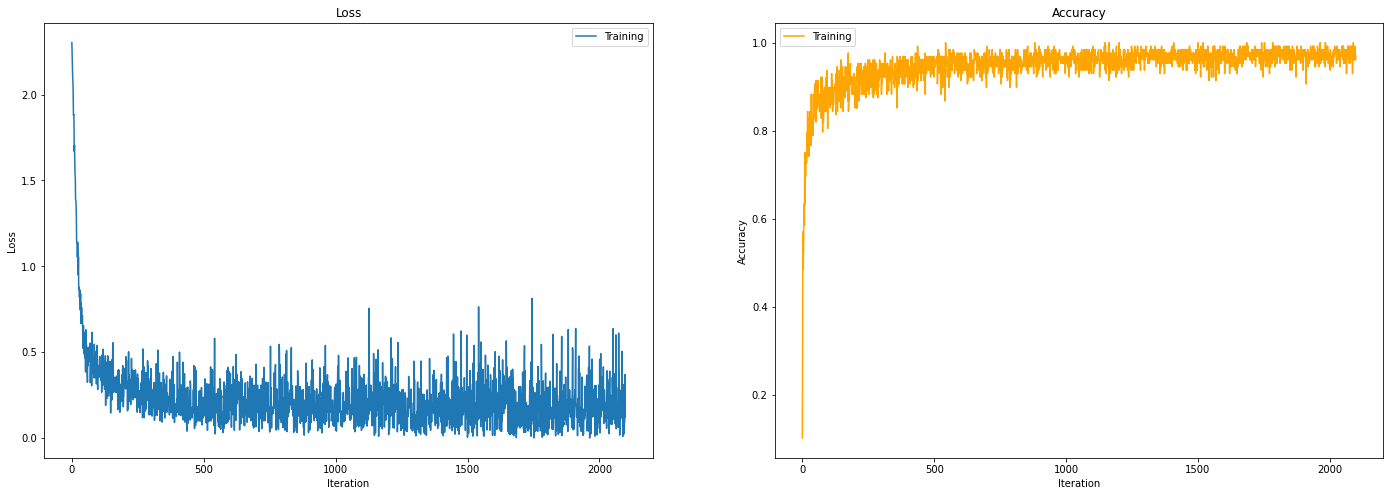
\includegraphics[width=0.9\textwidth]{./img/simple-board.png}
    \caption{Loss and Accuracy}
\end{figure}

Finally we test the network on the test dataset and get the accuracy \textbf{97.01\%}.

\bigskip

%------------------------------------------------

\section{\textbf{Modification}}

This part is some attempts to modify the original network architecture with some insights
from the assignment document, such as momentum, dropout, data augmentation, convolution
layers, etc. The code implementations are also in the jupyter notebook.

\subsection{\textbf{Change the Network Structure}}

In this section, we focus on both number of hidden units and number of hidden layers. We
first fix the number of hidden layers to 1, and then change the number of hidden units
accordingly. To avoid the overfitting, we test the network \textbf{every epoch}. Here is
the result:

\begin{table}[H]
    \begin{center}
        \begin{tabular}{cccccccccc}
            \toprule
            Units & 7      & 8      & 9      & 10     & 11     & 12              & 13              & 14              & 15              \\
            \midrule
            64    & 0.9703 & 0.9718 & 0.973  & 0.9744 & 0.974  & 0.9753          & 0.9762          & 0.9767          & \textbf{0.9767} \\
            128   & 0.9695 & 0.972  & 0.9738 & 0.9741 & 0.9738 & 0.975           & \textbf{0.9756} & 0.9738          & 0.9754          \\
            256   & 0.9696 & 0.9706 & 0.9736 & 0.9743 & 0.9734 & 0.9736          & 0.9734          & \textbf{0.9758} & 0.9744          \\
            512   & 0.9686 & 0.9707 & 0.9708 & 0.9718 & 0.9725 & \textbf{0.9738} & 0.9735          & 0.9737          & 0.9731          \\
            \bottomrule
        \end{tabular}
        \caption{Number of Hidden Units}
    \end{center}
\end{table}

We can see that there is no significant difference between the accuracy of the network with
64, 128, 256 and 512 hidden units. One thing need to be noted is that network with 64 hidden
units is not able to converge to the best accuracy due to the limited max epochs. Consequently,
maybe there's \textbf{no monotonous relationship} between the number of hidden units and final
accuracy.

Secondly, we try the network with 2 hidden layers, and units for each layer is 256, 64 in order.

\begin{table}[H]
    \begin{center}
        \begin{tabular}{cccccccccc}
            \toprule
            6      & 7      & 8      & 9     & 10    & 11     & 12     & 13     & 14     & 15              \\
            \midrule
            0.9527 & 0.9586 & 0.9661 & 0.965 & 0.967 & 0.9698 & 0.9719 & 0.9733 & 0.9734 & \textbf{0.9741} \\
            \bottomrule
        \end{tabular}
        \caption{Deeper Network}
    \end{center}
\end{table}

Same situation as the 64 hidden units network, the max epochs for this network is not enough.
However, as trying more training epochs, we encountered the problem of \textbf{dividing by zero}
in log softmax, this is weird because it never happens before.

To put it into a nutshell, the network structure has \textbf{no significant impact} on the
accuracy in MNIST classification task, at least the relationship between them is not simply
"the more complex the better". And when it comes to more complicated network, you may meet
other problems such as not enough training epochs.

\subsection{\textbf{Momentum in SGD}}

Momentum is a technique that can help the network to converge faster. In this section, we
try momentum to train the network. The core code is in the following code snippet:

\begin{lstlisting}
class SGD(Optimizer):
    """SGD with momentum."""

    def __init__(
        self, params: List['Tensor'], lr: float = 1e-3, momentum: float = 0.9
    ) -> None:
        super().__init__(params, lr)
        self.momentum = momentum
        self.v = [np.zeros(param.shape) for param in self.params]

    def step(self) -> None:
        for param, v in zip(self.params, self.v):
            v = self.momentum * v + self.lr * param.grad
            param.data = param.data - v
\end{lstlisting}

Thus by setting the parameter momentum to 0 or 0.9, we experiment the effect of momentum in
SGD optimizer. Here is the result:

\begin{figure}[H]
    \centering
    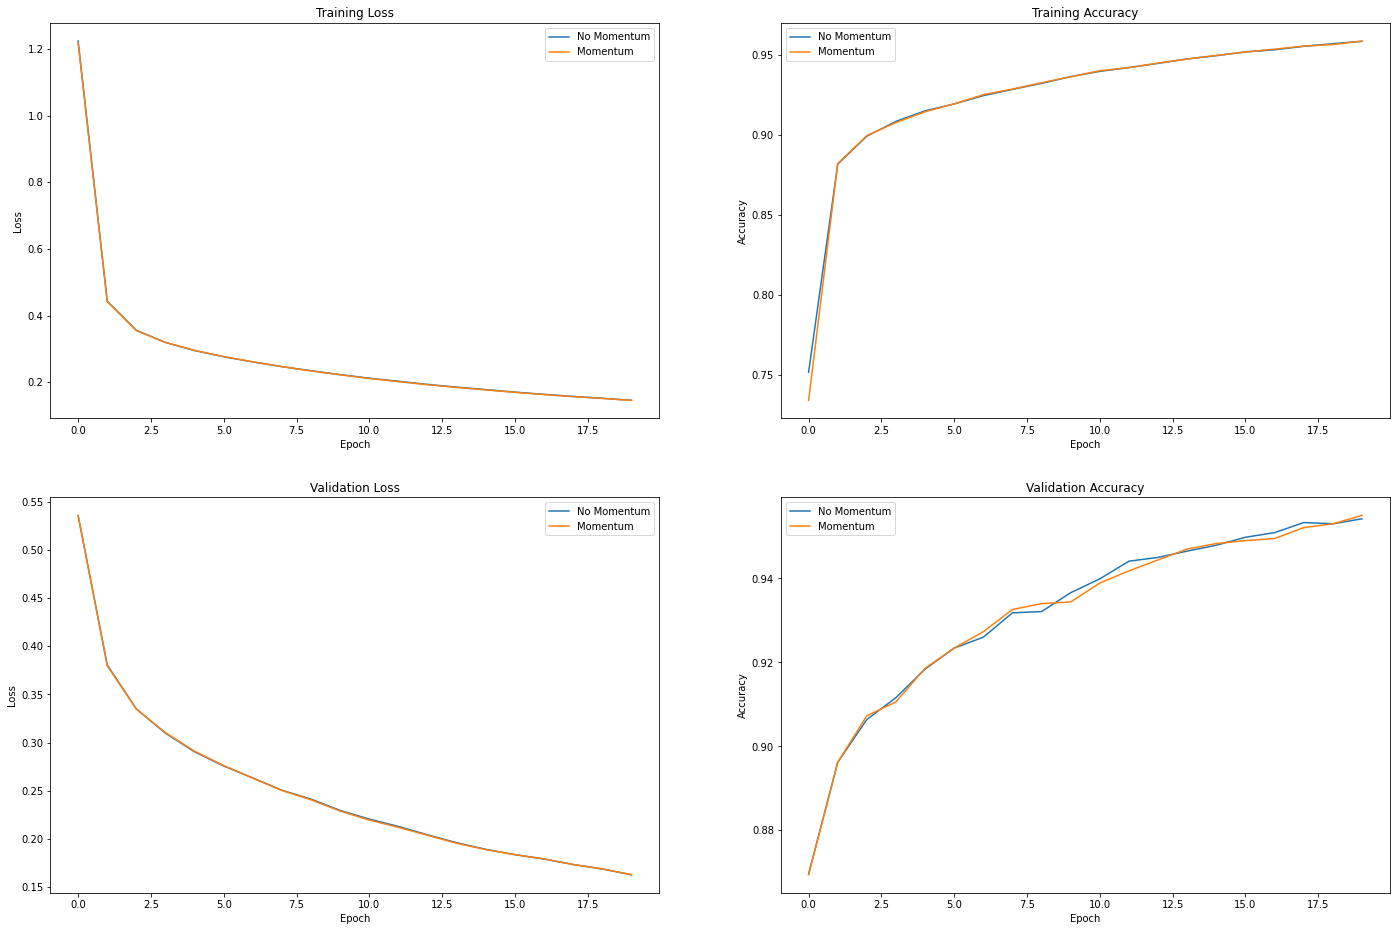
\includegraphics[width=0.9\textwidth]{./img/momentum.png}
    \caption{Momentum Effect}
\end{figure}

The test accuracy is almost equal (\textbf{95.72\%} with momentum 0.9 and \textbf{95.77\%}
without momentum). We know momentum \textbf{absorbs the gradient} of the previous step,
which means the network will have \textbf{inertia} in converging. Therefore, this inertia
may not be a good thing in preliminary stage but when the network is in the final stage,
this inertia definitely \textbf{accelerate the convergence}.

\subsection{\textbf{Vectorization}}

Vectorization is a classical technique to accelerate the matrix computation. As our whole
framework is built on numpy, we already implement vectorization implicitly. So we can skip
this section, just keep in mind that vectorization is faster than for loops, splendidly!

\subsection{\textbf{Regularization \& Early Stopping}}

Regularization is easy to implement, and it is a good idea to avoid overfitting. However,
before implementing regularization, we decide to plot the weights of toy model in heatmap
first to see whether there are outliers.

\begin{figure}[H]
    \centering
    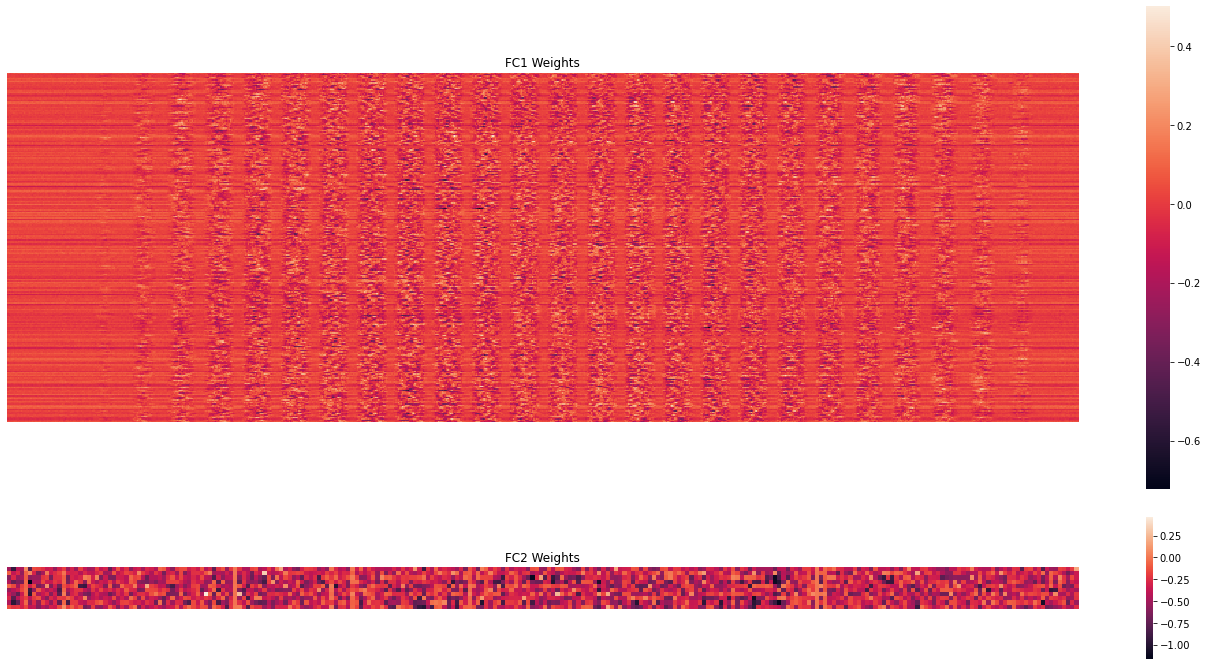
\includegraphics[width=0.9\textwidth]{./img/hearmap.png}
    \caption{Heatmap of Weights}
\end{figure}

As we can observe, the \textbf{range of weights} meets the expectation, and there is no
outlier.

The code snippet for regularization is as follows:

\begin{lstlisting}
class SGD(Optimizer):
    """SGD with momentum."""

    def __init__(
        self,
        params: List['Tensor'],
        lr: float = 1e-3,
        momentum: float = 0.9,
        weight_decay: float = 0.0,
    ) -> None:
        super().__init__(params, lr, weight_decay)
        self.momentum = momentum
        self.v = [np.zeros(param.shape) for param in self.params]

	def step(self) -> None:
        for param, v in zip(self.params, self.v):
            v = self.momentum * v + self.lr * param.grad

            if not param.is_bias:
                param.data = (
                    param.data
                    - v
                    - self.weight_decay
                    * param.data
                    / np.linalg.norm(param.data, ord='fro')
                )
            # Bias is not regularized
            else:
                param.data = param.data - v


class Adam(Optimizer):
	def __init__(
		self,
		params: List['Tensor'],
		lr: float = 1e-3,
		weight_decay: float = 0.0,
		beta1: float = 0.9,
		beta2: float = 0.999,
		eps: float = 1e-8,
	) -> None:
		super().__init__(params, lr, weight_decay)
		self.beta1 = beta1
		self.beta2 = beta2
		self.m = [np.zeros(param.shape) for param in self.params]
		self.v = [np.zeros(param.shape) for param in self.params]
		self.t = 0  # number of steps
		self.eps = eps

	def step(self) -> None:
        self.t += 1
        lr_t = self.lr * np.sqrt(1 - self.beta2 ** self.t) / (1 - self.beta1 ** self.t)
        eps = self.eps * self.t ** 0.5
        for param, m, v in zip(self.params, self.m, self.v):
            m = self.beta1 * m + (1 - self.beta1) * param.grad
            v = self.beta2 * v + (1 - self.beta2) * param.grad ** 2

            if not param.is_bias:
                param.data = (
                    param.data
                    - lr_t * m / (np.sqrt(v) + eps)
                    - self.weight_decay
                    * param.data
                    / np.linalg.norm(param.data, ord='fro')
                )
            # Bias is not regularized
            else:
                param.data = param.data - lr_t * m / (np.sqrt(v) + eps)
\end{lstlisting}

After attempting the regularization with setting the weight decay to 0.01, the test accuracy
\textbf{doesn't improve much}, this result is not surprising since the heatmap shows that the
weights are not too far from the mean.

Next is early stopping, the code snippet is simple as follows:

\begin{lstlisting}
# Early stopping
trigger_times = 0
patience = 2

max_epochs = 10
train_losses = []
val_losses = [100]  # Initialize with a huge loss

for epoch in range(max_epochs):
	# Training stage (skip)

	# Validation stage(skip)

	# Early stopping
	if val_losses[-1] > val_losses[-2]:
        trigger_times += 1
        if trigger_times == patience:
            print("Early Stopping!")
            print(f'\tTraining Losses: {train_losses}')
            print(f'\tValidation Losses: {val_losses[1:]}')
            break
    else:
        trigger_times = 0
\end{lstlisting}

\begin{figure}[H]
    \centering
    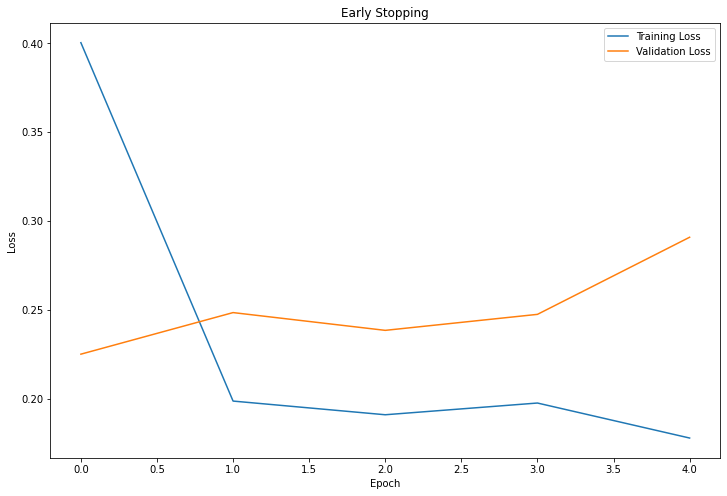
\includegraphics[width=0.6\textwidth]{./img/early-stopping.png}
    \caption{Early Stopping}
\end{figure}

The training process stops when the validation loss is increasing for a certain number of
epochs, here we set default to 2. And as we can see from the figure, early stopping appears
at 5th epoch out of 10 epochs. The test result is \textbf{96.97\%}, not bad!

\subsection{\textbf{Softmax}}

Referring to PyTorch's nn.CrossEntropyLoss, we combine \textbf{log softmax} and
\textbf{negative log likelihood loss} in a single function as follows:

\begin{lstlisting}
class CrossEntropyLoss(Function):
    """Combines log_softmax and nll_loss in a single function."""

    def __repr__(self) -> str:
        return 'Function(CrossEntropyLoss)'

    def forward(self, input: 'Tensor', target: 'Tensor') -> 'Tensor':
        self.save_backward_node([input, target])
        m = input.shape[0]
        input_data = input.data
        target_data = target.data

        # softmax = exp(x[target]) / sum(exp(x[i]), axis=1)
        neg_log_softmax = -input_data[np.arange(m), target_data] + np.log(
            np.sum(np.exp(input_data), axis=1)
        )

        return Tensor(
            np.mean(neg_log_softmax), grad_fn=self, requires_grad=input.requires_grad
        )

    def backward(self, out: np.ndarray) -> None:
        a, b = self.prev
        m = a.shape[0]
        input_data = a.data
        target_data = b.data

        # neg_log_softmax' = softmax - 1 * (i == target)
        softmax = np.exp(input_data) / np.sum(np.exp(input_data), axis=1).reshape(-1, 1)
        softmax[np.arange(m), target_data] -= 1
        a.grad = softmax / m
\end{lstlisting}

By training models in identical structure with same data batchs, we can fairly compare the
performance of different loss functions. By the way, in order to amplify the difference,
we use SGD instead of Adam.

\begin{figure}[H]
    \centering
    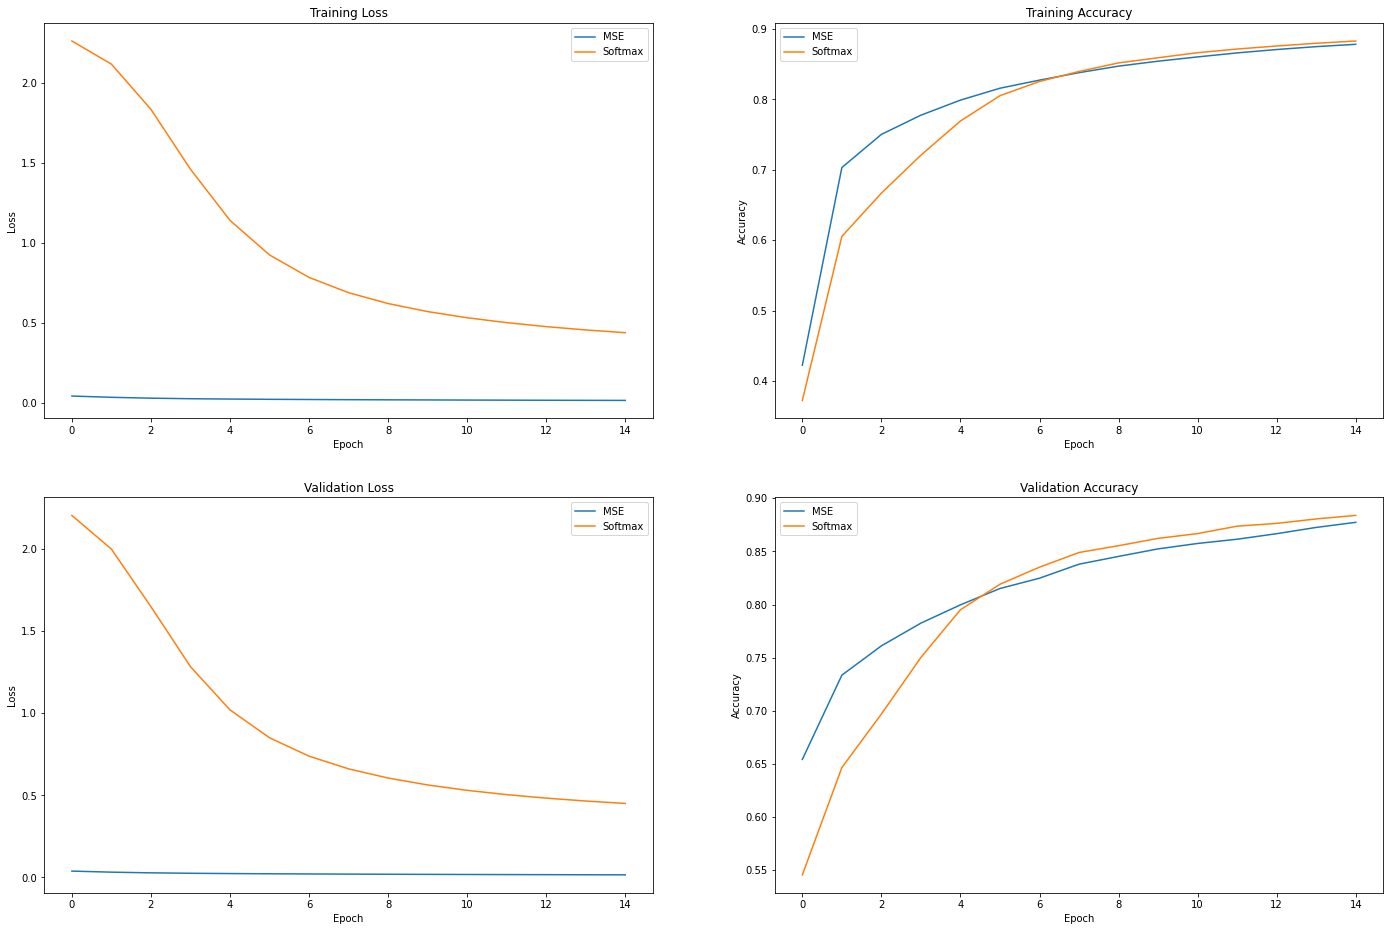
\includegraphics[width=0.9\textwidth]{./img/loss-function.png}
    \caption{Loss Function Comparison}
\end{figure}

And the final results for MSELoss and CrossEntropyLoss are close too (\textbf{89.25\%} and
\textbf{89.23\%} respectively). Although they are both in their way to converge, we can
still find some macro laws, like the \textbf{training loss} of CrossEntropyLoss is much
greater than that of MSELoss, which could be verified by simple examples. In this situation,
CrossEntropyLoss would gain \textbf{greater gradient} than MSELoss, so as to make the
training process more efficient.

So we just claim that \textbf{CrossEntropyLoss} is a better loss function for classification
tasks.

\subsection{\textbf{Bias}}

The linear layer module is designed to have the interface of bias in advance, like:

\begin{lstlisting}
class Linear(Module):
    def __init__(self, in_features: int, out_features: int, bias: bool = True) -> None:
        super().__init__()
        self.weight = Tensor(
            np.random.randn(in_features, out_features) * 0.01, requires_grad=True
        )

        if bias:
            self.bias = Tensor(np.zeros((1, out_features)), requires_grad=True)
            self._params.extend([self.weight, self.bias])
        else:
            self.bias = None
            self._params.append(self.weight)

    def __repr__(self) -> str:
        return f'Linear({self.weight.shape[0]}, {self.weight.shape[1]}, \
			bias={self.bias is not None})'

    def forward(self, input: 'Tensor') -> 'Tensor':
        if self.bias is not None:
            return input.dot(self.weight) + self.bias  # x @ W + b
        else:
            return input.dot(self.weight)  # x @ W
\end{lstlisting}

Here follows the comparison of whether bias or not in the linear layer module. In addition,
we choose SGD optimizer to slow down the convergence, intended to make the training process
more detailed.

\begin{figure}[H]
    \centering
    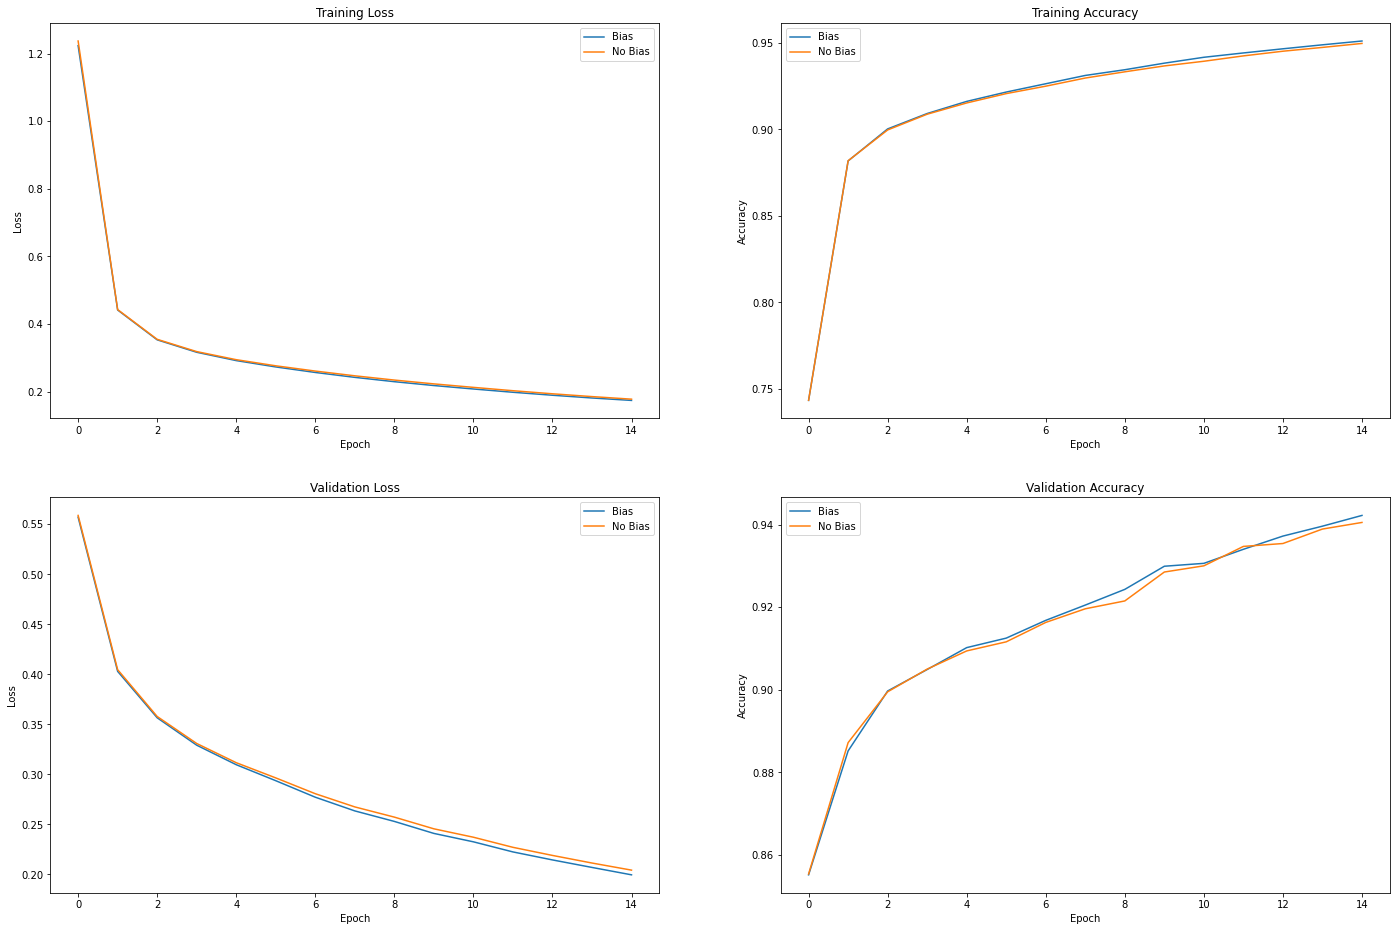
\includegraphics[width=0.9\textwidth]{./img/bias.png}
    \caption{Bias Effect}
\end{figure}

As we can see, they behave similarly and ultimately come up with same result, in test dataset
they perform accuracies \textbf{95.24\%} (with bias) and \textbf{95.00\%} (without bias),
very closely.

Consequently we guess the \textbf{bias is not a big deal} in this situation.

\subsection{\textbf{Dropout}}

During training, the Dropout layer \textbf{randomly zeroes} some of the elements of the input
tensor \textbf{with probability p} using samples from a Bernoulli distribution. Each channel
will be zeroed out independently on every forward call. Furthermore, the outputs are \textbf{scaled}
by a factor of $\frac{1}{1-p}$.

\begin{lstlisting}
class Dropout(Function):
    def __init__(self, p: float = 0.5, training: bool = True) -> None:
        super().__init__()
        self.p = p
        self.training = training
        self.mask = None

    def __repr__(self) -> str:
        return 'Function(Dropout)'

    def forward(self, a: 'Tensor') -> 'Tensor':
        if self.training:
            self.save_backward_node([a])
            out = a.data
            self.mask = np.random.binomial(1, self.p, size=a.shape) / (1 - self.p)
            out = out * self.mask
            return Tensor(out, grad_fn=self, requires_grad=a.requires_grad)

        else:
            return Tensor(a.data, grad_fn=self, requires_grad=a.requires_grad)

    def backward(self, out: np.ndarray) -> None:
        a = self.prev[0]
        a.grad = self.mask * out
\end{lstlisting}

\begin{figure}[H]
    \centering
    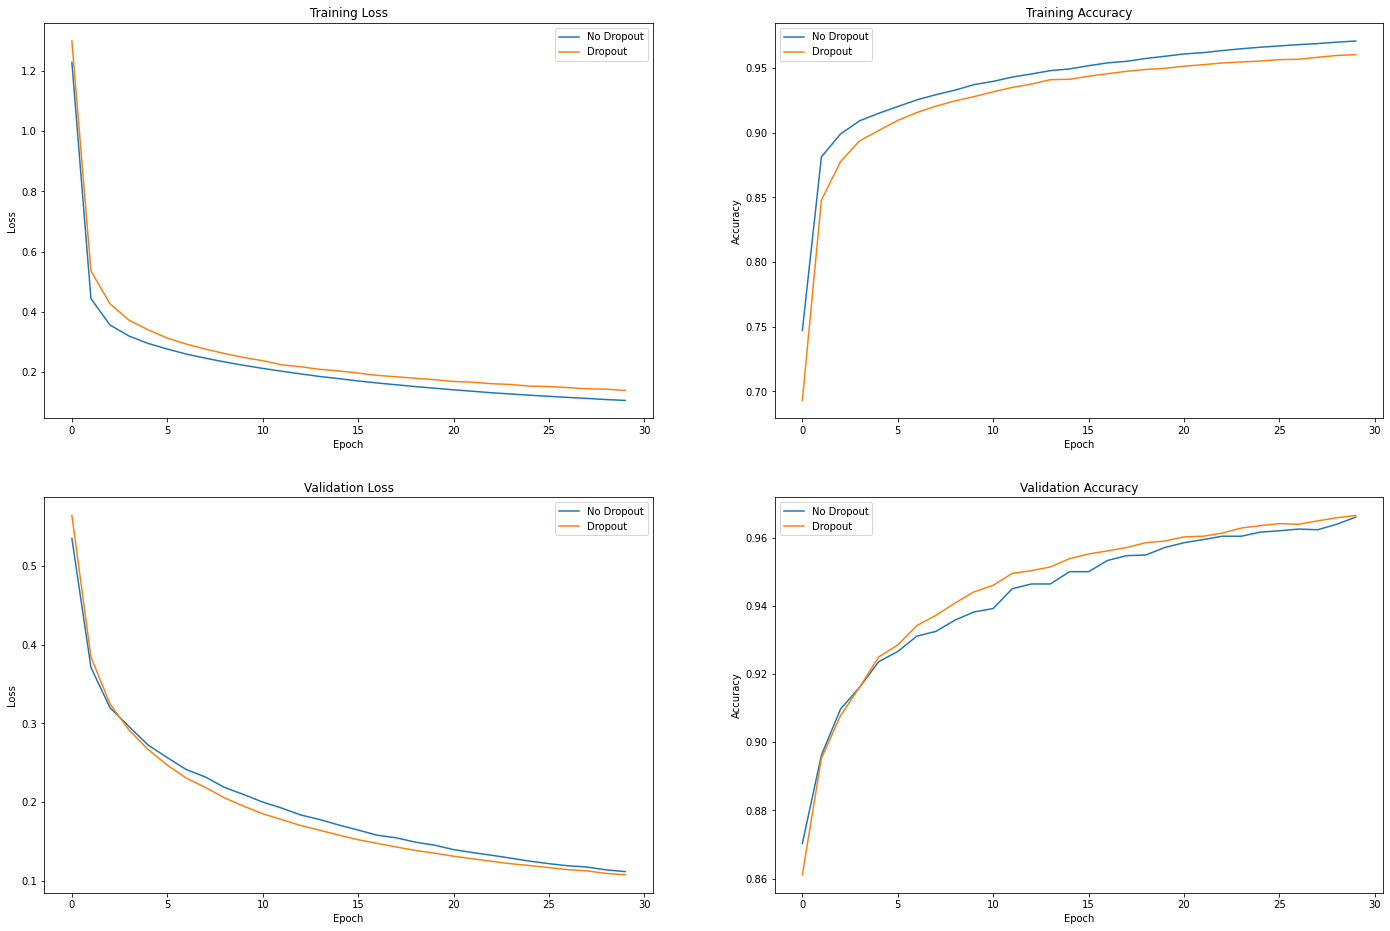
\includegraphics[width=0.9\textwidth]{./img/dropout.png}
    \caption{Dropout Effect}
\end{figure}

The effect of Dropout is that the model is less sensitive to the noise and the training
process is more \textbf{stable}. However, experiments show that Dropout \textbf{helps little}
in this task (We have tried $p=0.2,0.5,0.7$, figure above is case of $p=0.5$). The accuracies
are \textbf{96.73\%} (with Dropout) and \textbf{96.67\%} (without Dropout).

\subsection{\textbf{Fine Tuning}}

Fine tuning is tailor-made for \textbf{MSELoss}, our code implements like this:

\begin{lstlisting}
# * Fine tuning
fc2_bias_data = model_finetune.fc2.bias.data
x_ft = np.concatenate(x_ft)
y_ft = np.concatenate(y_ft)
x_ft_mpinv = np.matmul(
    np.linalg.pinv(np.matmul(x_ft.T, x_ft)), x_ft.T
)  # Moore-Penrose pseudoinverse
fc2_weight_data = np.matmul(
    x_ft_mpinv, (y_ft - fc2_bias_data)
)  # (X^T * X)^-1 * X^T * (Y - b)
model_finetune.fc2.weight.data = fc2_weight_data
\end{lstlisting}

However this time, we are pleasantly surprised by the result. The accuracy of the model with
fine tuning is \textbf{97.11\%} while the other without fine tuning is only \textbf{95.83\%},
seems fine tuning really helps \textbf{improve the converging speed}.

\begin{figure}[H]
    \centering
    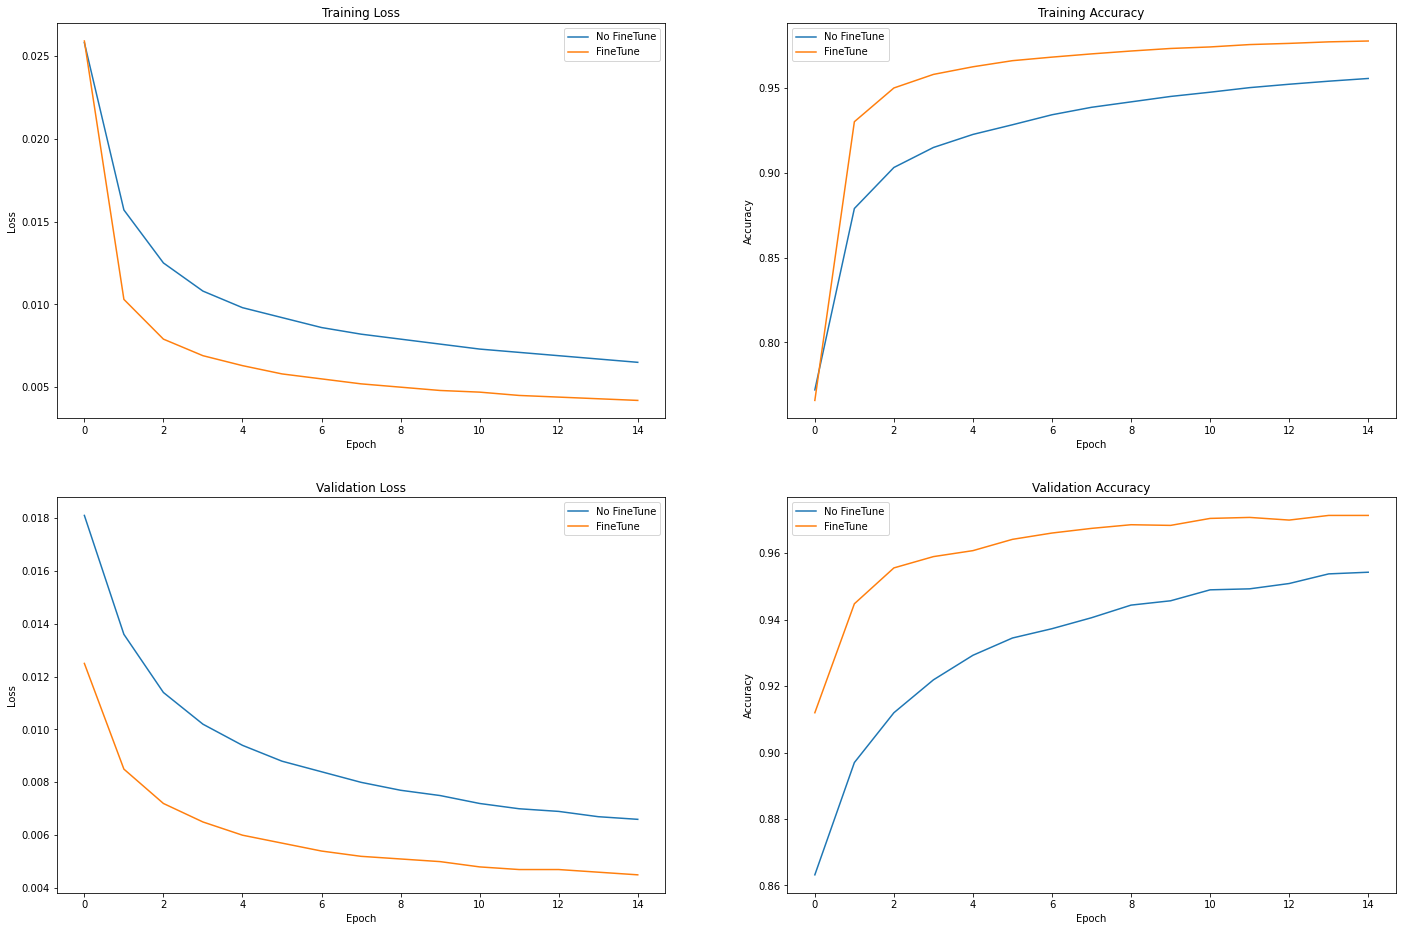
\includegraphics[width=0.9\textwidth]{./img/finetuning.png}
    \caption{Fine Tuning}
\end{figure}

\subsection{\textbf{Data Augmentation}}

Referring to torchvision.transforms, we implement data augmentation like normalize, resize,
crop, rotate, etc.

\begin{lstlisting}
size = 32  # Format support: (h, w) or k for (k, k)
mnist_transform = T.Compose([T.Resize(size), T.ToTensor(), T.Normalize((0.1307,), (0.3081,))])
mnist_train = dsets.MNIST(mnist_root, train=True, transform=mnist_transform)
\end{lstlisting}

\begin{figure}[H]
    \centering
    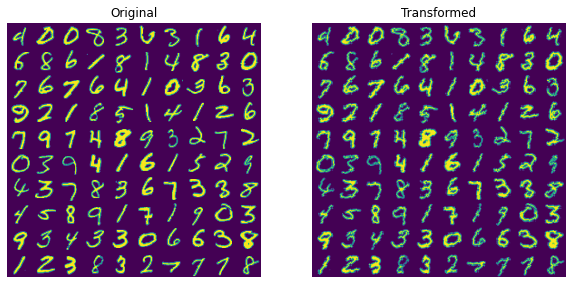
\includegraphics[width=0.6\textwidth]{./img/resize.png}
    \caption{Resize Illustration}
\end{figure}

\begin{lstlisting}
size = 16  # Format support: (h, w) or k for (k, k)
mnist_transform = T.Compose([T.CenterCrop(size), T.ToTensor(), T.Normalize((0.1307,), (0.3081,))])
mnist_train = dsets.MNIST(mnist_root, train=True, transform=mnist_transform)
\end{lstlisting}

\begin{figure}[H]
    \centering
    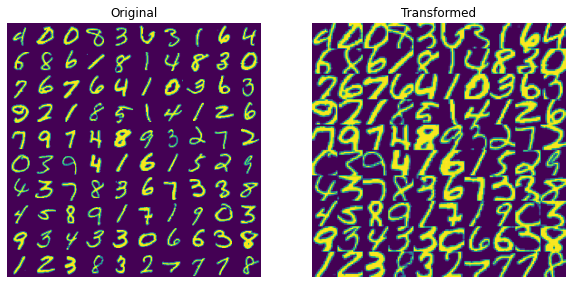
\includegraphics[width=0.6\textwidth]{./img/centercrop.png}
    \caption{CenterCrop Illustration}
\end{figure}

\begin{lstlisting}
size = 20  # Format support: (h, w) or k for (k, k)
mnist_transform = T.Compose([T.RandomResizedCrop(size), T.ToTensor(), T.Normalize((0.1307,), (0.3081,))])
mnist_train = dsets.MNIST(mnist_root, train=True, transform=mnist_transform)
\end{lstlisting}

\begin{figure}[H]
    \centering
    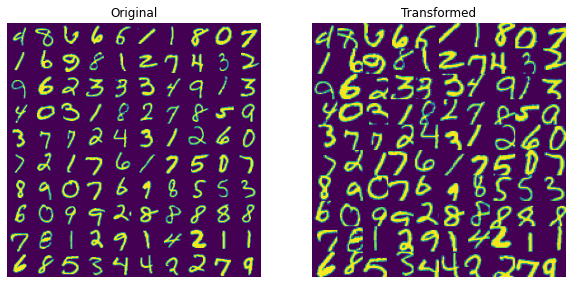
\includegraphics[width=0.6\textwidth]{./img/randomresize.png}
    \caption{RandomResizedCrop Illustration}
\end{figure}

\begin{lstlisting}
radians = (-np.pi / 4, np.pi / 4)  # Conter-clockwise is positive
mnist_transform = T.Compose([T.RandomRotation(radians), T.ToTensor(), T.Normalize((0.1307,), (0.3081,))])
mnist_train = dsets.MNIST(mnist_root, train=True, transform=mnist_transform)
\end{lstlisting}

\begin{figure}[H]
    \centering
    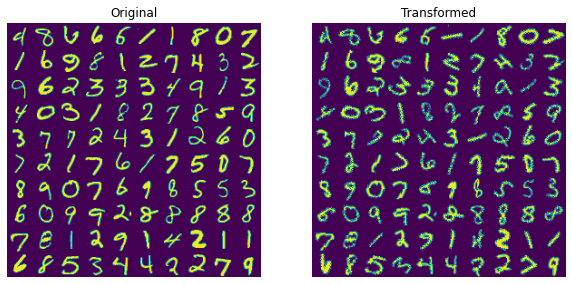
\includegraphics[width=0.6\textwidth]{./img/randomrotate.png}
    \caption{RandomRotation Illustration}
\end{figure}

After setting to different transforms, we find that the training result does not improve much.
Maybe the original dataset is \textbf{already sufficiently complete}.

\subsection{\textbf{Convolutional Layer}}

Convolutional layer is one of the most powerful layers in deep learning, it can be used to
\textbf{extract features} from the input data. An illustration of convolution operation is
shown below:

\begin{figure}[H]
    \centering
    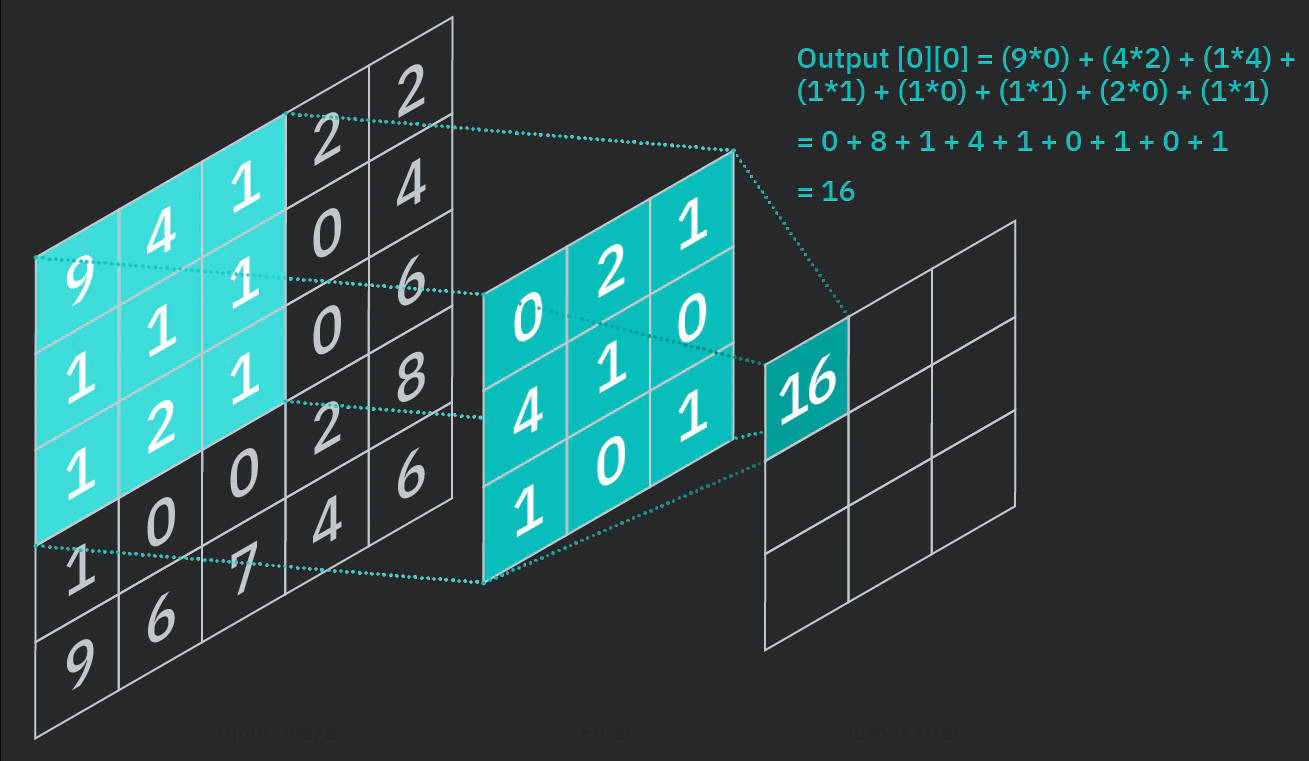
\includegraphics[width=0.6\textwidth]{./img/conv.jpg}
    \caption{Convolution Operation}
\end{figure}

Here is partial code of convolution operation:

\begin{lstlisting}
class Conv2d(Module):
    def __init__(
        self,
        in_channels: int,
        out_channels: int,
        kernel_size: Tuple[int, ...],
        stride: Tuple[int, ...] = (1, 1),
        padding: Tuple[int, ...] = (0, 0),
        bias: bool = True,
    ) -> None:
        super().__init__()
        self.in_channels = in_channels
        self.out_channels = out_channels
        self.kernel_size = _pair(kernel_size)
        self.stride = _pair(stride)
        self.padding = _pair(padding)

        # Initialize weight and bias
        scale = np.sqrt(
            2.0 / (self.in_channels * self.kernel_size[0] * self.kernel_size[1])
        )
        self.weight = Tensor(
            np.random.randn(self.out_channels, self.in_channels, *self.kernel_size)
            * scale,
            requires_grad=True,
        )
        if bias:
            self.bias = Tensor(
                np.zeros((1, self.out_channels, 1, 1)),
                requires_grad=True,
                is_bias=True,
            )
            self._params.extend([self.weight, self.bias])
        else:
            self.bias = None
            self._params.append(self.weight)

    def forward(self, input: 'Tensor') -> 'Tensor':
        return F.conv2d(input, self.weight, self.bias, self.stride, self.padding)
\end{lstlisting}

And the result shows that network with convolutional layer can be trained much faster than
network with only linear layer. The accuracies on test dataset are \textbf{97.21\%} and
\textbf{96.34\%} respectively.

\begin{figure}[H]
    \centering
    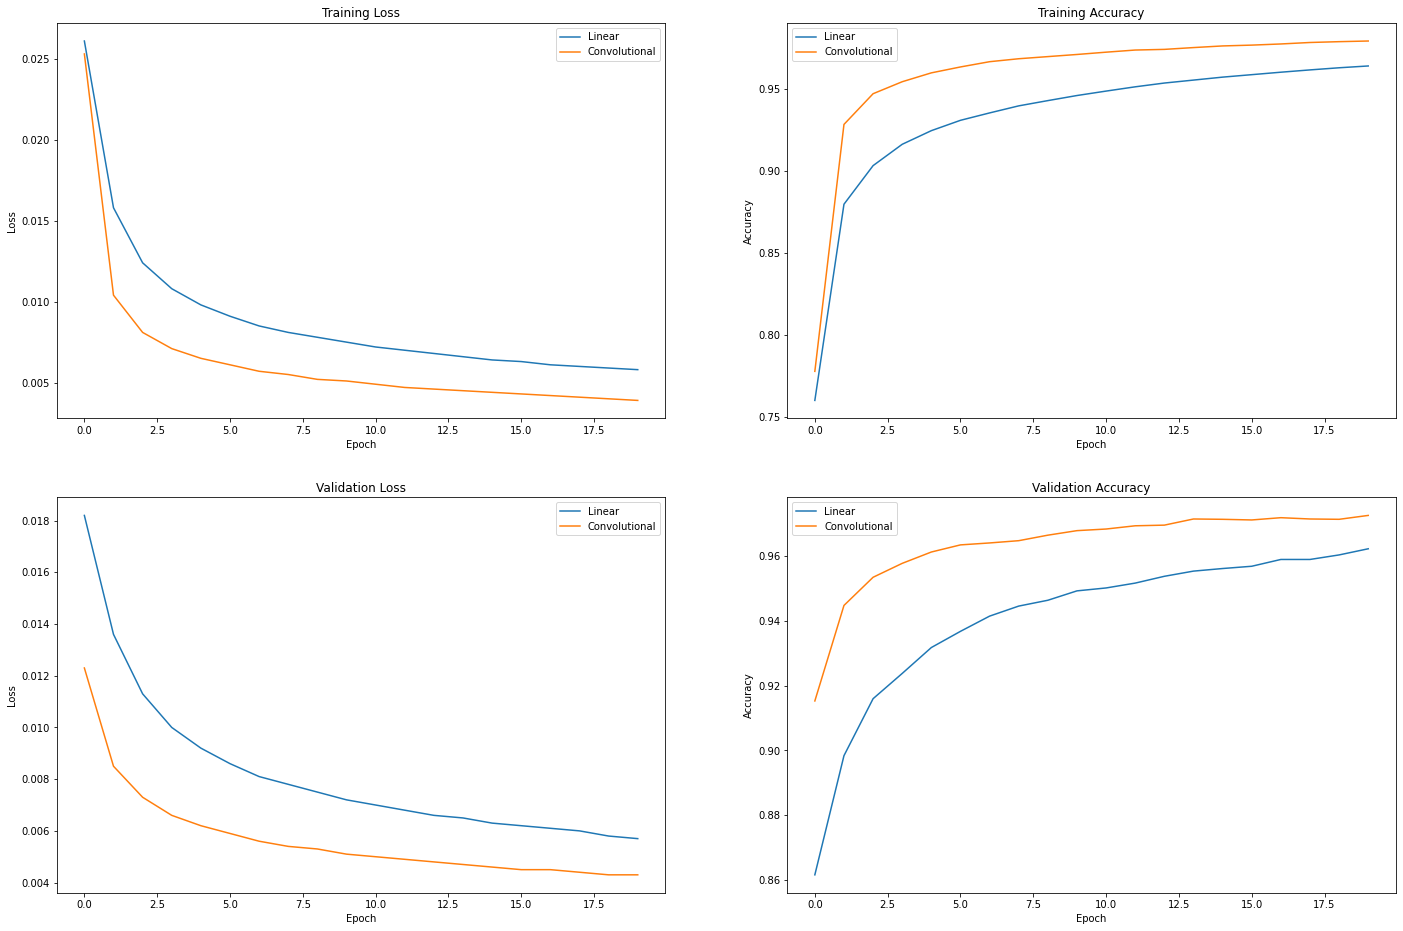
\includegraphics[width=0.9\textwidth]{./img/conv-layer.png}
    \caption{Convolutional Layer}
\end{figure}

\bigskip

%----------------------------------------------------------------------------------------
%	REFERENCE LIST
%----------------------------------------------------------------------------------------

% \cite{Eureka}
% \printbibliography

%----------------------------------------------------------------------------------------

\end{document}
